\chapter{Traitement des données et conception de l'intelligence artificielle}

\section{Introduction}
Dans le chapitre précédent, nous avons exploré la création d'une plateforme de visualisation des données. Ce chapitre se concentre sur le traitement des données collectées et la conception d'un modèle d'intelligence artificielle. Nous détaillerons les étapes nécessaires pour préparer les données, sélectionner et optimiser le modèle, et évaluer ses performances. L'objectif est de rendre les données exploitables pour l'entraînement du modèle et d'assurer une prédiction précise des paramètres clés des batteries.

\subsection{Traitement des données}
\subsubsection{Collecte des données}
Il est essentiel de normaliser les données collectées, car elles peuvent contenir du bruit. Les données brutes mesurées sont les suivantes :
\begin{itemize} 
	\item La tension 
	\item Le courant 
	\item La température
	\item SoC
	\item DoD
 \end{itemize}

Pour obtenir ces données, nous avons réalisé une collecte durant un cycle de charge et de décharge d'une batterie Lithium NMC-LCO 18650, d'une capacité nominale de 2,8 Ah et d'une tension nominale de 3,7 V, en appliquant un courant de charge et de décharge. Les caractéristiques complètes de la batterie se trouvent dans l'annexe. 

Les données collectées sont transmises par l'ESP32 et stockées dans la base de données pour être visualisées et utilisées par la plateforme, ainsi que pour la prédiction et l'entraînement du modèle. Voici, dans cette image, un aperçu de la table qui contient les données :

\begin{figure}[H]
	\centering
	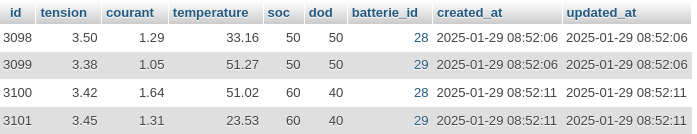
\includegraphics[width=17cm]{./img/tableLecture.png}
	\caption{Table dans la base de données ( Lectures )}
\end{figure}

\subsubsection{Nettoyage des données}
Les données brutes collectées peuvent contenir des erreurs, des incohérences ou des valeurs aberrantes dues à des défauts des capteurs, des interférences environnementales ou des problèmes de communication. Ces erreurs peuvent fausser les analyses, les prévisions et les conclusions tirées.

Définir une plage nominale afin de filtrer les valeurs qui se trouvent en dehors de ces limites.



\begin{table}[H]
	\centering
	\caption{Plage des valeurs acceptables}
	\begin{tabular}{|p{5cm}|p{5cm}|}
		\hline
		\textbf{Paramètre} & \textbf{Plage} \\
		\hline
		Tension & 2.75V - 4.2V \\
		\hline
		Courant & 1.4A - 4.2A \\
		\hline
		Température & 0°C à 60°C \\
		\hline
		SOC & 0\% à 100\% \\
		\hline
		DOD & 0\% à 100\% \\
		\hline
	\end{tabular}
\end{table}

Les données manquantes peuvent provenir de pannes de capteurs, interruptions réseau ou autres problèmes techniques. Pour y remédier, plusieurs méthodes sont utilisées :

\subsubsection{Gestion des valeurs manquantes}

\begin{itemize}
	\item \textbf{Imputation (remplacement des valeurs manquantes)}
	\begin{itemize}
		\item \textbf{Moyenne / Médiane (Température des batteries) :} Remplace une valeur manquante par la moyenne ou médiane des valeurs voisines.
		
		\textbf{Exemple :} Si la température à $t = 10s$ est absente, elle est estimée par la moyenne des valeurs à $t = 9s$ et $t = 11s$.
		
		\item \textbf{Interpolation (Tension et courant) :} Estime une valeur manquante à partir des mesures avant et après.
		
		\textbf{Exemple :} Si la tension à $t = 6s$ est absente, elle peut être estimée par une interpolation linéaire entre $3.3V$ ($t = 5s$) et $3.5V$ ($t = 7s$), donnant :
		
		\[
		V(6s) = \frac{3.3V + 3.5V}{2} = 3.4V
		\]
	\end{itemize}
	
	\item \textbf{Suppression des données incomplètes}
	
	Si plus de 50\% des données sont manquantes, l’enregistrement est supprimé pour éviter les biais.
	
	\textbf{Exemple :} Un SoC mesuré sur 10 instants, dont 6 valeurs sont manquantes, est jugé non fiable et ignoré.
	
	\item \textbf{Réduction du bruit et détection des anomalies}
	\begin{itemize}
		\item \textbf{Filtre de Kalman (Tension et courant) :} Lisse les variations et améliore la précision des mesures.
		
		\textbf{Exemple :} Si la tension passe brutalement de $3.5V$ à $10V$, le filtre corrige cette incohérence en tenant compte des valeurs précédentes.
	\end{itemize}
\end{itemize}
\subsection{Définition des nouveaux paramètres}
Les nouveaux paramètres sont obtenus grâce à des méthodes de traitement des données et des calculs spécifiques, également connus sous le nom d'ingénierie des features. Ces paramètres sont particulièrement adaptés pour l'entraînement de modèles et la prédiction des performances des batteries, en permettant une analyse plus approfondie de leur comportement au cours des cycles de charge et de décharge.

\begin{table}[H]
	\centering
	\caption{Définition des nouveaux paramètres}
	\begin{tabular}{|p{6cm}|p{9cm}|}
		\hline
		\textbf{Paramètre} & \textbf{Description} \\
		\hline
		\textbf{Cycle} & Nombre de cycles complets de charge et de décharge effectués par la batterie \\
		\hline
		\textbf{Temps de décharge/charge} & Durée totale des phases de charge et de décharge (en secondes) \\
		\hline
		\textbf{Tension de décharge/charge} & Tension mesurée pendant la phase de charge ou de décharge \\
		\hline
		\textbf{Courant de décharge/charge} & Courant circulant lors des phases de charge et de décharge \\
		\hline
		\textbf{Tension max. en décharge (V)} & Tension maximale atteinte au cours de la décharge \\
		\hline
		\textbf{Tension min. en charge (V)} & Tension minimale atteinte au cours de la charge \\
		\hline
		\textbf{RUL} & Estimation de la durée de vie restante de la batterie \\
		\hline
		\textbf{SOH} & Indicateur de l'état de santé de la batterie, exprimant son efficacité par rapport à sa capacité initiale \\
		\hline
		\textbf{Température de décharge/charge} & Température de la batterie durant les cycles de charge et de décharge \\
		\hline
	\end{tabular}
\end{table}


\subsubsection*{Identifier les cycles de charge/décharge}
Un cycle de charge/décharge est défini comme une décharge complète suivie d'une recharge complète. On détecte un cycle en surveillant le SoC :

\begin{itemize}
	\item Décharge : \textbf{SoC diminue} de \textbf{100\%} vers \textbf{20\%} (ou un seuil bas défini).
	\item Charge : \textbf{SoC remonte} à \textbf{100\%}.
\end{itemize}

\subsubsection*{Calcul du temps de charge et de décharge}
\begin{itemize}
	\item \textbf{Temps de décharge} = Durée entre SoC\_max et SoC\_min.
	\item \textbf{Temps de charge} = Durée entre SoC\_min et SoC\_max.
\end{itemize}

\subsubsection*{Extraction de la tension min/max lors de la charge et de la décharge}
\begin{itemize}
	\item \textbf{Max Voltage en décharge} = Valeur maximale atteinte lors de la phase de décharge.
	\item \textbf{Min Voltage en charge} = Valeur minimale atteinte lors de la phase de charge.
\end{itemize}

%\subsubsection*{Calcul du temps en courant constant}
%Lors de la charge, le \textbf{courant reste constant} pendant un moment avant de diminuer (phase de saturation).

\subsubsection*{Calcul de la Capacité Actuelle}  
La capacité actuelle est obtenue en intégrant le courant de charge et de décharge au cours du temps :  

\begin{equation}
C_{\text{actuelle}} = C_{\text{initiale}} - \int I_{\text{décharge}}(t) \, dt
\end{equation}

où :  
\begin{itemize}
	\item $C_{\text{initiale}}$ est la capacité nominale de la batterie (en Ah),
	\item $I_{\text{décharge}}(t)$ est le courant de décharge instantané (en A),
	\item $dt$ est l'intervalle de temps de mesure.
\end{itemize}

En pratique, l'intégration est souvent effectuée de manière discrète par un microcontrôleur :  

\begin{equation}
C_{\text{actuelle}} = C_{\text{initiale}} - \sum I_{\text{décharge}}(t) \times \Delta t
\end{equation}

avec $\Delta t$ en heures pour que le résultat soit en Ah.

\subsubsection*{Estimation de la durée de vie restante (RUL)}
La \textbf{RUL} est une estimation du nombre de cycles restants avant la fin de vie de la batterie. Elle est basée sur la \textbf{capacité de la batterie} et son \textbf{taux de dégradation}.

\begin{equation}
RUL = \left( \frac{C_{\text{actuelle}}}{C_{\text{initiale}}} \right) \times \text{Nombre\_de\_cycles}
\end{equation}

où $\text{Nombre\_de\_cycles}$ représente le nombre total de cycles que la batterie peut supporter avant d'atteindre un seuil critique de capacité (par exemple, 80 \% de $C_{\text{initiale}}$).

\subsubsection*{Calcul du SOH (State of Health)}
Le \textbf{SOH}) mesure la capacité actuelle de la batterie par rapport à sa capacité initiale. Il est généralement exprimé en pourcentage et permet d’évaluer l'état de santé de la batterie.

\begin{equation}
SOH = \left( \frac{C_{\text{actuelle}}}{C_{\text{initiale}}} \right) \times 100
\end{equation}

Un \textbf{SOH de 100 \%} signifie que la batterie est en parfait état, tandis qu’un \textbf{SOH de 80 \% ou moins} indique une batterie vieillissante nécessitant un remplacement prochain.


\section{Modélisation} 
\subsection{Description des modèles}

Il existe plusieurs modèles que l'on peut explorer en Machine Learning, mais nous allons nous concentrer sur quelques-uns parmi les plus couramment utilisés, à savoir :

\begin{itemize}
	\item \textbf{Régression linéaire} : Modèle simple établissant une relation linéaire entre variables indépendantes et dépendante.
	\item \textbf{Régression de crête} : Variante de la régression linéaire avec pénalité L2 pour réduire la complexité et éviter le sur-apprentissage.
	\item \textbf{Régression Lasso} : Similaire à la régression de crête, mais avec pénalité L1, permettant la sélection automatique des caractéristiques.
	\item \textbf{Forêt aléatoire} : Ensemble d'arbres de décision réduisant le sur-apprentissage tout en maintenant une grande précision.
	\item \textbf{K-Plus proches voisins} : Modèle basé sur la proximité des données, avec la sortie déterminée par les k voisins les plus proches.
	\item \textbf{Réseaux de neurones artificiels} : Modèles inspirés du cerveau humain, capables de modéliser des relations complexes via des couches successives de neurones.
\end{itemize}

\subsubsection{R\'egression lin\'eaire (Linear Regression)}

La r\'egression lin\'eaire est un mod\`ele simple et largement utilis\'e en apprentissage automatique. Elle vise \`a mod\'eliser la relation entre une ou plusieurs variables ind\'ependantes \(X\) et une variable d\'ependante \(Y\) en ajustant une droite (ou un hyperplan en dimension sup\'erieure) minimisant l'erreur quadratique. L'\'equation du mod\`ele est :

\begin{equation}
Y = \beta_0 + \beta_1 X_1 + \beta_2 X_2 + \dots + \beta_n X_n
\end{equation}
O\`u :
\begin{itemize}
	\item \( Y \) : variable d\'ependante (valeur \`a pr\'edire).
	\item \( X_1, X_2, \dots, X_n \) : variables ind\'ependantes (pr\'edictives).
	\item \( \beta_0 \) : ordonn\'ee \`a l'origine.
	\item \( \beta_1, \beta_2, \dots, \beta_n \) : coefficients du mod\`ele \`a estimer.
\end{itemize}

\textbf{Avantages :}
\begin{itemize}
	\item Facile \`a impl\'ementer et interpr\'eter.
	\item Convient aux donn\'ees lin\'eairement s\'eparables.
	\item Exige peu de ressources de calcul.
\end{itemize}

\subsubsection{R\'egression de cr\^ete (Ridge Regression)}

La r\'egression de cr\^ete introduit une p\'enalit\'e L2 pour r\'eduire le sur-apprentissage en contraignant la magnitude des coefficients. La fonction de co\^ut devient :

\begin{equation}
J(\beta) = \sum_{i=1}^{m} (y_i - \hat{y}_i)^2 + \lambda \sum_{j=1}^{n} \beta_j^2
\end{equation}
O\`u :
\begin{itemize}
	\item \( y_i \) : valeur r\'eelle de l'observation \(i\).
	\item \( \hat{y}_i \) : valeur pr\'edite.
	\item \( \lambda \) : param\`etre de r\'egularisation (contr\^ole la p\'enalit\'e).
	\item \( \beta_j \) : coefficients du mod\`ele.
\end{itemize}

\textbf{Avantages :}
\begin{itemize}
	\item R\'eduit le risque de sur-apprentissage.
	\item Convient aux donn\'ees ayant de fortes corr\'elations entre les variables.
\end{itemize}

\subsubsection{R\'egression Lasso (Lasso Regression)}

La r\'egression Lasso applique une p\'enalit\'e L1, ce qui permet la s\'election de variables en annulant certains coefficients. La fonction de co\^ut est :


\begin{equation}
\hat{C} = \sum_{i=1}^{m} (y_i - \hat{y}_i)^2 + \lambda \sum_{j=1}^{n} |\beta_j|
\end{equation}

\textbf{Avantages :}
\begin{itemize}
	\item Permet la s\'election automatique des variables les plus importantes.
	\item R\'eduit la complexit\'e du mod\`ele en mettant certains coefficients \`a z\'ero.
\end{itemize}

\subsubsection{For\^et al\'eatoire (Random Forest)}

La for\^et al\'eatoire est un mod\`ele d'ensemble bas\'e sur plusieurs arbres de d\'ecision. Chaque arbre est entra\^in\'e sur un sous-ensemble al\'eatoire du jeu de donn\'ees. La pr\'ediction finale est obtenue par agr\'egation :



\begin{equation}
\hat{y} = \frac{1}{n_{arbres}} \sum_{i=1}^{n_{arbres}} f_i(X)
\end{equation}

\textbf{Avantages :}
\begin{itemize}
	\item Pr\'ecision \'elev\'ee et robuste \`a l'overfitting.
	\item Convient aux relations non lin\'eaires.
	\item G\'ere les donn\'ees bruit\'ees et les valeurs manquantes.
\end{itemize}

\subsubsection{K-Plus Proches Voisins (K-Nearest Neighbors, KNN)}

KNN pr\'edit une valeur en utilisant les \(K\) plus proches voisins d'un point dans l'espace des caract\'eristiques. Pour une r\'egression, la pr\'ediction est la moyenne :

\begin{equation}
\hat{y} = \frac{1}{K} \sum_{i=1}^{K} y_i
\end{equation}
\textbf{Avantages :}
\begin{itemize}
	\item Simple \`a comprendre et \`a impl\'ementer.
	\item Fonctionne bien pour des donn\'ees locales complexes.
	\item Pas besoin d'hypoth\`ese sur la distribution des donn\'ees.
\end{itemize}

\subsubsection{R\'eseaux de neurones artificiels (Artificial Neural Networks, ANN)}

Les r\'eseaux de neurones sont compos\'es de couches de neurones interconnect\'es. Chaque neurone applique une fonction d'activation \`a une somme pond\'er\'ee des entr\'ees :

\begin{equation}
Z^{(l)} = W^{(l)} a^{(l-1)} + b^{(l)}
\end{equation}

\begin{equation}
a^{(l)} = f(Z^{(l)})
\end{equation}



\textbf{Avantages :}
\begin{itemize}
	\item Excellente capacit\'e \`a mod\'eliser des relations non lin\'eaires complexes.
	\item Adapt\'e aux grands jeux de donn\'ees et aux probl\`emes multi-dimensionnels.
	\item Am\'eliorable avec des techniques comme le deep learning.
\end{itemize}


\subsection{Critères d'évaluation des modèles de régression}

\subsubsection{Erreur Quadratique Moyenne (MSE)}
\begin{equation}
MSE = \frac{1}{n} \sum_{i=1}^{n} (y_i - \hat{y}_i)^2
\end{equation}
\textbf{Interprétation :} 

Plus la valeur du MSE est faible, plus le modèle est précis. Cependant, il est très sensible aux valeurs aberrantes, car il élève les erreurs au carré.
\begin{itemize}
	\item MSE = 0 : modèle parfait, aucune erreur.
	\item MSE > 0 : le modèle présente des erreurs, avec une erreur plus grande pour des valeurs plus élevées.
\end{itemize}

\subsubsection{Erreur Absolue Moyenne (MAE)}
\begin{equation}
MAE = \frac{1}{n} \sum_{i=1}^{n} |y_i - \hat{y}_i|
\end{equation}
\textbf{Interprétation :} 

Le MAE représente l'erreur moyenne en valeur absolue. Il est moins sensible aux valeurs aberrantes que le MSE, mais ne met pas autant en évidence les grandes erreurs.
\begin{itemize}
	\item MAE = 0 : modèle parfait, aucune erreur.
	\item MAE > 0 : le modèle présente des erreurs proportionnelles à la magnitude de l'erreur absolue.
\end{itemize}

\subsubsection{Erreur Quadratique Moyenne Racine (RMSE)}
\begin{equation}
RMSE = \sqrt{MSE} = \sqrt{\frac{1}{n} \sum_{i=1}^{n} (y_i - \hat{y}_i)^2}
\end{equation}
\textbf{Interprétation :} 

Le RMSE permet d'obtenir une erreur moyenne dans la même unité que la variable cible, facilitant son interprétation par rapport au MSE.
\begin{itemize}
	\item RMSE = 0 : modèle parfait, aucune erreur.
	\item RMSE > 0 : le modèle présente des erreurs, et plus la valeur est grande, plus les erreurs sont importantes.
\end{itemize}

\subsubsection{Coefficient de Détermination ($R^2$)}
\begin{equation}
R^2 = 1 - \frac{\sum (y_i - \hat{y}_i)^2}{\sum (y_i - \bar{y})^2}
\end{equation}
\textbf{Interprétation :} 

Le $R^2$ indique la proportion de la variance expliquée par le modèle. Une valeur proche de 1 signifie que le modèle ajuste bien les données, tandis qu'une valeur proche de 0 indique un faible pouvoir explicatif.
\begin{itemize}
	\item $R^2 = 1$ : modèle parfait, explique toute la variance des données.
	\item $R^2 = 0$ : le modèle n'offre aucune amélioration par rapport à la moyenne, il n'explique aucune variance.
	 \item $R^2 < 0$ : la prédiction est inférieure à la moyenne, les résultats sont moins précis que la simple moyenne des valeurs cibles.
\end{itemize}


\subsection{Validation des modèles de régression}

\subsubsection{Validation croisée (Cross-Validation)}
\textbf{Principe :} la validation croisée consiste à diviser l'ensemble de données en plusieurs sous-ensembles ou "folds". À chaque itération, un sous-ensemble est utilisé comme jeu de test, tandis que les autres sous-ensembles servent à l'entraînement du modèle. Cette procédure permet de mesurer la performance du modèle de manière plus robuste, en réduisant le risque de surapprentissage (overfitting).
\begin{itemize}
	\item \textbf{k-Fold Cross-Validation :} diviser l'ensemble de données en $k$ sous-ensembles égaux, puis entraîner le modèle $k$ fois, chaque fois en utilisant un sous-ensemble différent comme jeu de test. L'erreur moyenne sur les $k$ itérations est calculée comme suit :
	
	\begin{equation}
	\text{Score moyen} = \frac{1}{K} \sum_{k=1}^{K} \text{Score}_k
	\end{equation}
	où :
	\begin{itemize}
		\item $K$ : représente le nombre total de plis (ou "folds") dans la validation croisée.
		\item $\text{Score}_k$ : représente le score de performance pour le $k$-ième pli.
		\item Les données sont divisées en $K$ sous-ensembles égaux.
		\item Le modèle est entraîné sur $K-1$ sous-ensembles et testé sur le sous-ensemble restant.
		\item Ce processus est répété $K$ fois, chaque sous-ensemble servant de test une fois.
		\item Le score moyen est calculé en prenant la moyenne des scores de performance obtenus sur chaque pli.
	\end{itemize}
	
%	\subsubsection*{Time Series Split :}
%	\begin{itemize}
%		\item Adapté aux séries temporelles, où les données sont divisées en plis successifs en respectant l'ordre chronologique.
%		\item Cela évite la contamination des données de test par les données futures.
%		\item Le score moyen est calculé de manière similaire en prenant la moyenne des scores de performance pour chaque pli, en respectant l'ordre temporel.
%	\end{itemize}

\end{itemize}

\subsubsection{Courbe d'apprentissage}
\textbf{Principe :} les courbes d'apprentissage permettent de suivre l'évolution de la performance du modèle au fur et à mesure de l'entraînement. Elles sont particulièrement utiles pour détecter les problèmes de surapprentissage ou de sous-apprentissage.
\begin{itemize}
	\item \textbf{Surapprentissage (Overfitting) :} si la performance du modèle sur le jeu d'entraînement continue de s'améliorer tandis que celle sur le jeu de test se dégrade, cela indique un surapprentissage.
	\item \textbf{Sous-apprentissage (Underfitting) :} si le modèle ne parvient pas à bien ajuster à la fois le jeu d'entraînement et le jeu de test, cela peut indiquer un sous-apprentissage, où le modèle est trop simple pour capturer les relations dans les données.
\end{itemize}

\subsubsection{Évaluation sur un jeu de test indépendant}
\textbf{Principe :} après avoir entraîné le modèle sur un sous-ensemble des données (jeu d'entraînement), il est important d'évaluer sa performance sur un jeu de test indépendant qui n'a pas été utilisé pendant l'entraînement. Cela permet de s'assurer que le modèle est capable de généraliser et de faire des prédictions fiables sur des données non vues.
\begin{itemize}
	\item Un jeu de test indépendant permet d'éviter le biais d'évaluation dû au surapprentissage sur les données d'entraînement.
\end{itemize}


\section{Développement et implémentation}
 \subsection{Outils} Durant le développement, en particulier pour le traitement des données, l'entraînement et le test du modèle, nous avons utilisé la plateforme en ligne Google Colab, qui est gratuite. Elle facilite l'installation des frameworks et des bibliothèques nécessaires au développement, telles que :

\begin{itemize} 
	\item pandas 
	\item NumPy 
	\item Scikit-learn 
	\item TensorFlow 
	\item Keras 
\end{itemize}

\section{Phases de prédiction}

L'objectif est de créer un modèle entraîné capable de prédire les paramètres suivants : 
\begin{itemize} 
	\item SOH : état de santé de la batterie 
	\item RUL : nombre de cycles restants de la batterie \end{itemize}

Voici l'organigramme illustrant le processus de prédiction : 


\begin{figure}[H]
	\centering
	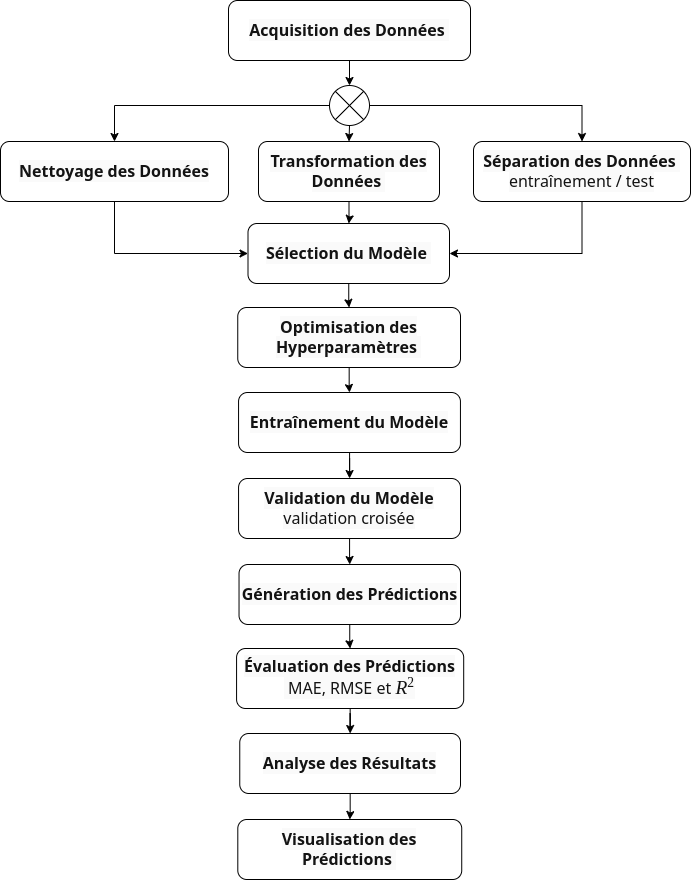
\includegraphics[width=12cm]{./img/processus.png}
	\caption{Organigramme du processus de prédiction}

\end{figure}


\subsection{Acquisition des données}

Nous importons le fichier "battery\_data\_collecter.csv" ici pour pouvoir l'utiliser dans notre travail.

\begin{minted}[frame=single,framesep=8pt]{python}

from google.colab import files
uploaded = files.upload() 
data = pd.read_csv('battery_data_collecter.csv')
print(data.head())

\end{minted}

\textbf{Résultats}
\begin{figure}[H]
	\centering
	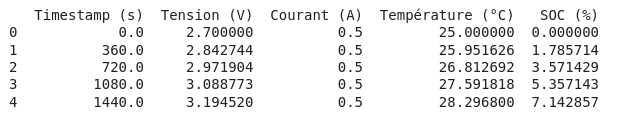
\includegraphics[width=16cm]{./img/resultats/loadData.png}
    \caption{Affichage du résultat du chargement des données collectées brutes}

\end{figure}


\subsection{Nettoyage des données}
Suppression des valeurs manquantes et des doublons, suivie de l’élimination des valeurs aberrantes à l’aide de la méthode de l’écart interquartile (IQR).
\begin{minted}[frame=single,framesep=8pt]{python}

# Fonction pour identifier et filtrer les valeurs aberrantes
def remove_outliers(df):
   for column in df.select_dtypes(include=[np.number]).columns:
     Q1 = df[column].quantile(0.25)
     Q3 = df[column].quantile(0.75)
     IQR = Q3 - Q1
     lower_bound = Q1 - 1.5 * IQR
     upper_bound = Q3 + 1.5 * IQR
     # Filtrer les valeurs aberrantes
     df = df[(df[column] >= lower_bound) & (df[column] <= upper_bound)]
   return df
	
# 1. Suppression des valeurs manquantes
data_cleaned = data.dropna()
	
# 2. Suppression des doublons
data_cleaned = data_cleaned.drop_duplicates()
	
# 3. Identification et traitement des valeurs aberrantes
data_cleaned = remove_outliers(data)
	
# Vérifier la structure des données après nettoyage
print(data_cleaned.describe())
\end{minted}
\textbf{Résultats}
\begin{figure}[H]
	\centering
	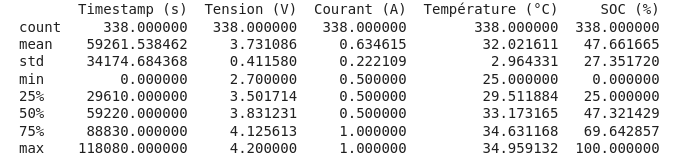
\includegraphics[width=16cm]{./img/resultats/netoyage.png}
	\caption{Affichage du résultat du nettoyage des données brutes collectées}
	
\end{figure}
\subsection{Transformation des données}
Les données sont transformées et normalisées afin d'obtenir de nouveaux paramètres essentiels pour le dataset, garantissant une meilleure qualité des données d'entraînement.
\begin{minted}[ frame=single, fontsize=\small, breaklines]{python}

#Transformation des Données
def calculate_cycle_summary(df, capacity_nominal, life_cycle_nominal=500):
  # Extraire les valeurs nécessaires du DataFrame
  soc_values = df['SOC (%)'].values
  timestamps = df['Timestamp (s)'].values
  tensions = df['Tension (V)'].values
  currents = df['Courant (A)'].values
  temperatures = df['Température (°C)'].values
  
  # Initialiser les variables pour le calcul
  total_discharge = 0
  charge_time = 0
  discharge_time = 0
  charge_tensions, discharge_tensions = [], []
  charge_currents, discharge_currents = [], []
  charge_temperatures, discharge_temperatures = [], []
  	
  # Parcourir les valeurs de SOC pour déterminer les phases de charge et de décharge
  for i in range(1, len(soc_values)):
    delta_soc = soc_values[i] - soc_values[i - 1]
    delta_time = timestamps[i] - timestamps[i - 1]
    
    if delta_soc > 0:  # Phase de charge
      charge_time += delta_time
      charge_tensions.append(tensions[i])
      charge_currents.append(currents[i])
      charge_temperatures.append(temperatures[i])
    elif delta_soc < 0:  # Phase de décharge
      discharge_time += delta_time
      total_discharge += abs(delta_soc)
      discharge_tensions.append(tensions[i])
      discharge_currents.append(currents[i])
      discharge_temperatures.append(temperatures[i])
  
  # Calculer le nombre total de cycles
  total_cycles = total_discharge / 100
  
  # Calculer les moyennes des tensions, courants et températures pendant les phases de charge et décharge
  avg_v_charge = sum(charge_tensions) / len(charge_tensions) if charge_tensions else 0
  avg_v_discharge = sum(discharge_tensions) / len(discharge_tensions) if discharge_tensions else 0
  avg_i_charge = sum(charge_currents) / len(charge_currents) if charge_currents else 0
  avg_i_discharge = sum(discharge_currents) / len(discharge_currents) if discharge_currents else 0
  avg_t_charge = sum(charge_temperatures) / len(charge_temperatures) if charge_temperatures else 0
  avg_t_discharge = sum(discharge_temperatures) / len(discharge_temperatures) if discharge_temperatures else 0
  
  # Trouver les valeurs maximales et minimales de tension pendant les phases de charge et décharge
  max_v_discharge = max(discharge_tensions) if discharge_tensions else 0
  min_v_charge = min(charge_tensions) if charge_tensions else 0
  	
  # Convertir le temps de décharge en heures
  discharge_time_h = discharge_time / 3600
  capacity_discharged = avg_i_discharge * discharge_time_h
  
  # Calculer le State of Health (SOH)
  soh = (capacity_discharged / (capacity_nominal * total_cycles)) * 100 if capacity_nominal and total_cycles > 0 else 0
  
  # Calculer le Remaining Useful Life (RUL)
  rul = (life_cycle_nominal * soh / 100) - total_cycles if total_cycles > 0 else life_cycle_nominal
  
  # Créer un DataFrame de résumé avec les résultats calculés
  summary_df = pd.DataFrame({
  	'Cycles': [total_cycles],
  	'T_charge (s)': [charge_time],
  	'T_discharge (s)': [discharge_time],
  	'V_charge (V)': [avg_v_charge],
  	'V_discharge (V)': [avg_v_discharge],
  	'V_max_dis (V)': [max_v_discharge],
  	'V_min_chg (V)': [min_v_charge],
  	'I_charge (A)': [avg_i_charge],
  	'I_discharge (A)': [avg_i_discharge],
  	'T°C_charge': [avg_t_charge],
  	'T°C_discharge': [avg_t_discharge],
  	'SOH (%)': [soh],
  	'RUL (cycles)': [rul]
  })
  return summary_df
\end{minted}


\subsection{Séparation des données}
Les données sont divisées en un ensemble d'entraînement (80 \%) et un ensemble de test (20 \%).
\begin{minted}[ frame=single, fontsize=\small, breaklines]{python}

  # Préparation des données pour l'entraînement et la normalisation
  # Séparation des variables cibles (RUL et SOH)
  y_rul = df['RUL (cycles)']
  y_soh = df['SOH (%)']
  
  # Suppression des colonnes cibles du jeu de données pour obtenir
   les entrées (features)
  x = df.drop(columns=['RUL (cycles)', 'SOH (%)'], axis=1)
  
  # Division des données en ensembles d'entraînement et de test (80% entraînement, 20% test)
  x_train, x_test, y_train_rul, y_test_rul = train_test_split(x, y_rul, test_size=0.20, random_state=42)
  _, _, y_train_soh, y_test_soh = train_test_split(x, y_soh, test_size=0.20, random_state=42)
  
  # Normalisation des données pour améliorer la performance des modèles
  scaler = StandardScaler()
  x_train = scaler.fit_transform(x_train)
  x_test = scaler.transform(x_test)
\end{minted}


\subsection{Sélection du modèle}
Lister les modèles sélectionnés pour l'entraînement, en les entraînant un par un afin de pouvoir comparer leurs performances.
\begin{minted}[ frame=single, fontsize=\small, breaklines]{python}

   # Définition d'un dictionnaire contenant différents modèles de régression
   
   models = {
   	# Régression linéaire simple
   	"Linear Regression": LinearRegression(),
   	# Régression Ridge avec régularisation 
   	"Ridge Regression": Ridge(alpha=0.1, random_state=42),
   	 # Régression Lasso avec régularisation
   	"Lasso Regression": Lasso(alpha=0.001, random_state=42)
   	# Modèle Random Forest optimisé 
   	"Random Forest (Optimized)": best_rf,
   	# Régression par plus proches voisins (KNN)
   	"K-Nearest Neighbors": KNeighborsRegressor(),
   	# Régression par réseau de neurones artificiels (MLP)  
   	"ANN Regression": MLPRegressor(hidden_layer_sizes=(256,), max_iter=1000, random_state=42)  
   }
\end{minted}


\subsection{Optimisation des hyperparamètres}
Ajustement des paramètres du modèle à l'aide de GridSearch, en définissant le nombre d'arbres, la profondeur maximale et le nombre minimal d'échantillons requis pour diviser un nœud.
\begin{minted}[ frame=single, fontsize=\small, breaklines]{python}

   # Recherche d'hyperparamètres avec GridSearchCV pour Random Forest
   # Définition des hyperparamètres à tester
   rf_params = {
   	'n_estimators': [50, 100, 200],  # Nombre d'arbres dans la forêt
   	'max_depth': [10, 20, None],  # Profondeur maximale des arbres
   	'min_samples_split': [2, 5, 10]  # Nombre minimum d'échantillons pour diviser un nœud
   }
   
   # Initialisation du modèle Random Forest
   rf = RandomForestRegressor(random_state=42)
   
   # GridSearchCV pour rechercher la meilleure combinaison d'hyperparamètres
   grid_search_rf = GridSearchCV(rf, rf_params, cv=5, scoring='r2', n_jobs=-1)
   
   # Entraînement du modèle avec GridSearchCV
   grid_search_rf.fit(x_train, y_train_rul)
   
   # Récupération du meilleur modèle après recherche des hyperparamètres
   best_rf = grid_search_rf.best_estimator_
   
   # Affichage des meilleurs hyperparamètres trouvés
   print(f"Meilleurs hyperparamètres pour Random Forest : {grid_search_rf.best_params_}")
\end{minted}
Affichage de résultat : 
\begin{figure}[H]
	\centering
	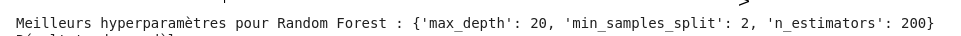
\includegraphics[width=16cm]{./img/resultats/goodParam.png}
	\caption{ Affichage des meilleurs hyperparamètres trouvés}
	
\end{figure}


\subsection{Entraînement du modèle}
Entraînement des modèles sur l'ensemble de données d'entraînement afin d'ajuster leurs paramètres et optimiser leurs performances.
\begin{minted}[frame=single, fontsize=\small, breaklines]{python}

   # Entraînement et évaluation des modèles
   # Liste pour stocker les résultats de performance des modèles
   results = []
   
   # Parcours de chaque modèle défini dans le dictionnaire "models"
   for name, model in models.items():
     # ----------------------
     # Entraînement et évaluation pour RUL (Remaining Useful Life)
     # ----------------------
     
     model.fit(x_train, y_train_rul)
     
     # Prédictions sur les ensembles d'entraînement et de test
     y_pred_train_rul = model.predict(x_train)
     y_pred_test_rul = model.predict(x_test)
     
     # Calcul des métriques de performance pour RUL
     metrics_rul = calculate_metrics(y_train_rul, y_test_rul, y_pred_train_rul, y_pred_test_rul)
     
     # Ajout d'informations sur le modèle et la cible dans les résultats
     metrics_rul['Model'] = name
     metrics_rul['Target'] = 'RUL (cycles)'
     
     # Validation croisée pour évaluer la robustesse du modèle
     metrics_rul['CrossVal R2'] = cross_val_score_model(model, x, y_rul)
     
     # Stockage des résultats pour RUL
     results.append(metrics_rul)
     
     # Enregistrement du modèle entraîné pour RUL
     joblib.dump(model, f'{name}_rul_model.pkl')
   
     # ----------------------
     # Entraînement et évaluation pour SoH (State of Health)
     # ----------------------
     
	 model.fit(x_train, y_train_soh)
	    
     # Prédictions sur les ensembles d'entraînement et de test
     y_pred_train_soh = model.predict(x_train)
     y_pred_test_soh = model.predict(x_test)
     
     # Calcul des métriques de performance pour SoH
     metrics_soh = calculate_metrics(y_train_soh, y_test_soh, y_pred_train_soh, y_pred_test_soh)
     
     # Ajout d'informations sur le modèle et la cible dans les résultats
     metrics_soh['Model'] = name
     metrics_soh['Target'] = 'SOH (%)'
     
     # Validation croisée pour évaluer la robustesse du modèle
     metrics_soh['CrossVal R2'] = cross_val_score_model(model, x, y_soh)
     
     # Stockage des résultats pour SoH
     results.append(metrics_soh)
     
     # Enregistrement du modèle entraîné pour SoH
     joblib.dump(model, f'{name}_soh_model.pkl')
   
   # Conversion des résultats en DataFrame pour une meilleure visualisation
   results_df = pd.DataFrame(results)
	
   # Affichage des résultats des modèles
   print("Résultats des modèles :\n", results_df)
\end{minted}


\subsection{Validation du modèle}
Évaluation du modèle à l'aide de techniques de validation croisée.
\begin{minted}[ frame=single, fontsize=\small, breaklines]{python}

	# Validation croisée pour évaluer le modèle
	def cross_val_score_model(model, x, y):
	scores = cross_val_score(model, x, y, cv=5, scoring='r2')
	return np.mean(scores)
\end{minted}

\subsection{Génération des prédictions}
Utilisation du modèle pour produire des prédictions.
\begin{minted}[ frame=single, fontsize=\small, breaklines]{python}

   # Normalisation des nouvelles données
   new_data_scaled = scaler.transform(new_data)
   
   # Stockage des prédictions
   predictions = []
   
   # Prédiction avec chaque modèle
   for name in models.keys():
      model_rul = joblib.load(f'{name}_rul_model.pkl')
      prediction_rul = model_rul.predict(new_data_scaled)
      
      model_soh = joblib.load(f'{name}_soh_model.pkl')
      prediction_soh = model_soh.predict(new_data_scaled)
      
      predictions.append({
      	'Model': name,
      	'Predicted RUL': prediction_rul[0],
      	'Predicted SoH': prediction_soh[0]
      })
   
   # Conversion en DataFrame et affichage
   predictions_df = pd.DataFrame(predictions)
   print("Prédictions :\n", predictions_df)
\end{minted}


\subsection{Évaluation des prédictions}
Mesure de la performance du modèle avec des métriques telles que MAE, RMSE et $R^2$.
\begin{minted}[ frame=single, fontsize=\small, breaklines]{python}

   # Fonction de calcul des métriques d'évaluation
   def calculate_metrics(y_train, y_test, y_pred_train, y_pred_test):
     return {
     	'MAE Train': mean_absolute_error(y_train, y_pred_train),
     	'MSE Train': mean_squared_error(y_train, y_pred_train),
     	'R2 Train': r2_score(y_train, y_pred_train),
     	'MAE Test': mean_absolute_error(y_test, y_pred_test),
     	'MSE Test': mean_squared_error(y_test, y_pred_test),
     	'R2 Test': r2_score(y_test, y_pred_test)
   }
\end{minted}


\subsection{Analyse des résultats}

Voici les images des résultats des métriques pendant l'entraînement et le test, suivies de la validation croisée.
\begin{figure}[H]
	\centering
	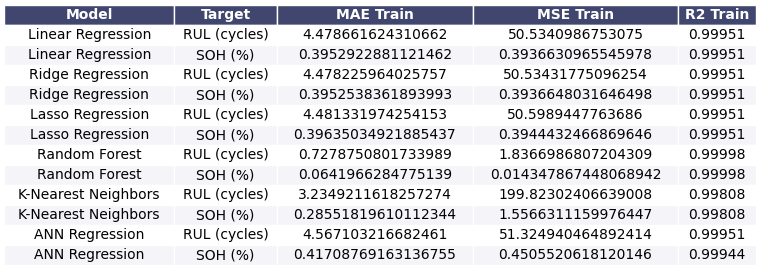
\includegraphics[width=17cm]{./img/resultats/Train.png}
	\caption{Résultats des métriques d'entraînement}
	\label{fig:train_metrics}
\end{figure}

\begin{figure}[H]
	\centering
	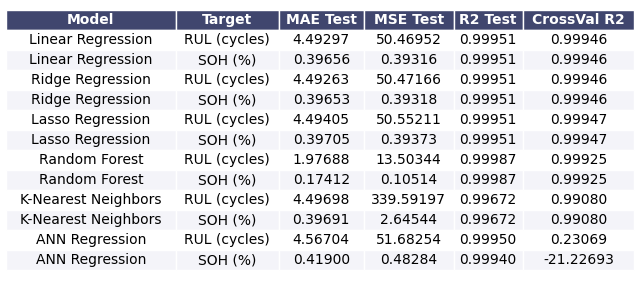
\includegraphics[width=17cm]{./img/resultats/train.png}
	\caption{Résultats des métriques de test et de validation croisée}
	\label{fig:test_validation_metrics}
\end{figure}

\subsubsection{Interprétation des résultats}

\subsubsection*{Prédiction du RUL (cycles)}
\begin{itemize}
	\item \textbf{Régressions linéaires (Linear, Ridge, Lasso) :} très bonnes performances avec $R^2 \approx 0.99951$, mais des erreurs (MAE, MSE) légèrement plus élevées que Random Forest.
	\item \textbf{Random Forest :} meilleure précision avec $R^2 = 0.99998$ et des erreurs extrêmement faibles.
	\item \textbf{K-Nearest Neighbors (KNN) :} performance inférieure avec $R^2 = 0.99808$ et des erreurs plus élevées.
	\item \textbf{ANN Regression :} bonne performance ($R^2 = 0.99951$), mais erreurs plus élevées que Random Forest.
\end{itemize}

\subsubsection*{Prédiction du SOH (\%)}
\begin{itemize}
	\item \textbf{Régressions linéaires :} similaires à RUL avec de très bonnes performances ($R^2 \approx 0.99951$), mais inférieures à Random Forest.
	\item \textbf{Random Forest :} meilleure précision avec $R^2 = 0.99998$ et des erreurs très faibles.
	\item \textbf{KNN :} performance inférieure avec $R^2 = 0.99808$ et erreurs plus élevées.
	\item \textbf{ANN Regression :} bonne capacité de prédiction ($R^2 = 0.99944$), mais moins précise que Random Forest.
\end{itemize}

\subsubsection*{Validation croisée}
\begin{itemize}
	\item \textbf{Random Forest :} excellente généralisation avec $R^2 = 0.99925$.
	\item \textbf{ANN Regression :} résultats incohérents en validation croisée, nécessitant une vérification.
\end{itemize}

\begin{itemize}
	\item \textbf{Random Forest est le modèle le plus performant} avec les meilleures valeurs de $R^2$ et les erreurs les plus faibles.
	\item \textbf{Les modèles de régression linéaire} sont solides mais légèrement moins précis.
	\item \textbf{KNN a les performances les plus faibles}, tandis qu'\textbf{ANN regression présente des résultats incohérents en validation croisée}.
\end{itemize}




\subsection{Visualisation des prédictions}
Création de graphiques pour visualiser les prédictions de consommation sur différentes périodes.
\begin{minted}[linenos, frame=single, fontsize=\small, breaklines]{python}

   # Visualisation des performances
   plt.figure(figsize=(12, 6))
   for target in ['RUL (cycles)', 'SOH (%)']:
     subset = results_df[results_df['Target'] == target]
     for metric in ['R2 Train', 'R2 Test', 'CrossVal R2']:
        plt.barh(subset['Model'], subset[metric], label=f'{metric} {target}')
   plt.title("Comparaison des performances des modèles")
   plt.xlabel("Score")
   plt.legend()
   plt.show()
\end{minted}

\subsection{Choix du model}
Le modèle \textbf{Random Forest} a été choisi pour plusieurs raisons clés, basées sur ses performances supérieures :

\subsubsection*{Performance}
\begin{itemize}
	\item \textbf{R² élevé} : le R² est très élevé pour l'entraînement et les tests, indiquant une forte capacité de prédiction pour RUL et SOH.
	\item \textbf{Faibles erreurs} : les erreurs absolue (MAE) et quadratique (MSE) sont faibles, surtout pour SOH, montrant des prédictions fiables.
\end{itemize}

\subsubsection*{Généralisation}
\begin{itemize}
	\item \textbf{Validation croisée} : le R² de validation croisée est élevé (0.99925), indiquant une bonne généralisation et minimisant le sur-apprentissage.
\end{itemize}

\subsubsection*{Comparaison avec d'autres modèles}
\begin{itemize}
	\item \textbf{Précision supérieure} : comparé à la régression linéaire et Ridge, Random Forest a une meilleure précision avec des MAE et MSE plus faibles pour RUL.
	\item \textbf{Meilleure performance} : par rapport à KNN et ANN, Random Forest a des erreurs plus faibles et une meilleure précision, notamment pour RUL.
\end{itemize}

\subsubsection*{Robustesse}
\begin{itemize}
	\item \textbf{Ensemble d'arbres} : random Forest est robuste aux variations de données et aux valeurs aberrantes, grâce à sa structure d'ensemble d'arbres de décision.
\end{itemize}
En résumé, \textbf{Random Forest} est préféré pour sa capacité à généraliser, ses faibles erreurs de prédiction, et ses excellentes performances en termes de R².
\section{Intégration}

Après avoir sélectionné le modèle optimal pour la prédiction du SOH et du RUL, nous téléchargeons les modèles entraînés :  

\begin{minted}[ frame=single, fontsize=\small, breaklines]{python}
   from google.colab import files
   
   # Télécharger les modèles entraînés depuis Google Colab
   files.download('Random Forest_rul_model.pkl')
   files.download('Random Forest_soh_model.pkl')
\end{minted}

Ensuite, nous transférons ces modèles vers le serveur hébergeant notre backend Laravel. Un script est mis en place pour exécuter les modèles et traiter les prédictions. De plus, un contrôleur spécifique et une route API dédiée sont implémentés pour intégrer ces prédictions au sein du système.  


\section{Conclusion}
Ce chapitre a exploré le traitement des données et la conception d'un modèle d'intelligence artificielle pour prédire le RUL et le SOH des batteries. Nous avons nettoyé et transformé les données, puis évalué plusieurs modèles de régression, notamment la régression linéaire, Ridge, Lasso, Random Forest, K-Nearest Neighbors, et les réseaux de neurones artificiels.

Le modèle Random Forest s'est distingué par ses performances supérieures, avec des valeurs de R² élevées et des erreurs faibles. Il a également montré une excellente capacité de généralisation grâce à la validation croisée.




























